\documentclass{article}


% if you need to pass options to natbib, use, e.g.:
%     \PassOptionsToPackage{numbers, compress}{natbib}
% before loading neurips_2023


% ready for submission
\usepackage{neurips_2023}


% to compile a preprint version, e.g., for submission to arXiv, add add the
% [preprint] option:
%     \usepackage[preprint]{neurips_2023}


% to compile a camera-ready version, add the [final] option, e.g.:
%     \usepackage[final]{neurips_2023}


% to avoid loading the natbib package, add option nonatbib:
%    \usepackage[nonatbib]{neurips_2023}


\usepackage[utf8]{inputenc} % allow utf-8 input
\usepackage[T1]{fontenc}    % use 8-bit T1 fonts
\usepackage{hyperref}       % hyperlinks
\usepackage{url}            % simple URL typesetting
\usepackage{booktabs}       % professional-quality tables
\usepackage{amsfonts}       % blackboard math symbols
\usepackage{nicefrac}       % compact symbols for 1/2, etc.
\usepackage{microtype}      % microtypography
\usepackage{xcolor}         % colors
\usepackage{graphicx}       % images


\title{Formatting Instructions For NeurIPS 2023}


% The \author macro works with any number of authors. There are two commands
% used to separate the names and addresses of multiple authors: \And and \AND.
%
% Using \And between authors leaves it to LaTeX to determine where to break the
% lines. Using \AND forces a line break at that point. So, if LaTeX puts 3 of 4
% authors names on the first line, and the last on the second line, try using
% \AND instead of \And before the third author name.


\author{%
  David S.~Hippocampus\thanks{Use footnote for providing further information
    about author (webpage, alternative address)---\emph{not} for acknowledging
    funding agencies.} \\
  Department of Computer Science\\
  Cranberry-Lemon University\\
  Pittsburgh, PA 15213 \\
  \texttt{hippo@cs.cranberry-lemon.edu} \\
  % examples of more authors
  % \And
  % Coauthor \\
  % Affiliation \\
  % Address \\
  % \texttt{email} \\
  % \AND
  % Coauthor \\
  % Affiliation \\
  % Address \\
  % \texttt{email} \\
  % \And
  % Coauthor \\
  % Affiliation \\
  % Address \\
  % \texttt{email} \\
  % \And
  % Coauthor \\
  % Affiliation \\
  % Address \\
  % \texttt{email} \\
}


\begin{document}


\maketitle


\begin{abstract}
  Chloe

  The abstract paragraph should be indented \nicefrac{1}{2}~inch (3~picas) on
  both the left- and right-hand margins. Use 10~point type, with a vertical
  spacing (leading) of 11~points.  The word \textbf{Abstract} must be centered,
  bold, and in point size 12. Two line spaces precede the abstract. The abstract
  must be limited to one paragraph.

  A short description of your goals, task, model, and (for
the final report) results. The abstract should make the
motivations and the scope of your project clear so that
readers can decide whether they are interested in
reading your work.
\end{abstract}


\section{Introduction}
% Gabriel

% A description of the motivation behind your work, why
% the task you chose is interesting/important, and a
% summary of your (proposed) approach. The problem
% that you want to solve should be clearly stated in the
% introduction: especially the input and output of your
% model and the format of the input and output. This
% section should also make it clear why your deep
% learning approach is reasonable for this problem.
A challenge often faced by students in the computational sciences is learning how to solve logically intensive math questions. Often times the transition from computation focused math to reasoning focused math presents a large learning curve due to the difficulty of developing mathematical intuition and a lack of rigorous step by step answers to compare with. We hope to develop an accessible model that can take in a latex text input of a math problem and output a descriptive and accurate latex text answer output to the problem. Developing models capable of solving this task is an infamously difficult problem (\href{https://arxiv.org/html/2410.02666v1}{https://arxiv.org/html/2410.02666v1}) due to the requirement of consistency and mathematical riqour within the answers outputted by the models. Currently the best models in this area use transformer LLM archetictures with large pretraining datasets. The downsides of these models is that the consistency may be poor due to multiple ways to present the same problem which are treated differently by the model. To solve for this we are incorporating a symbolic model into a transformer LLM architecture to hopefully increase accuracy within our math solving model. We believe this deep learning approach is reasonable as understanding the language of math problems is something suited for transformer LLM models and creating consistency in mathematical reasoning is something that symbolic models are good at. By combining these 2 approaches we hope that it will combine the best of both architectures.  With this work we hope to develop a more robust and helpful model that is able to answer with reason and provide thorough feedback on math questions potential users might have.

\section{Background and related work}
Chloe

A summary of the background material that students of
CSC413 would not already be familiar with. A
description of related work done in the area, and how
your approach compares with theirs.

If your project builds on previous work, clearly
distinguish what they did from what your new
contribution is. Also, include a 1-2 sentence summary
of other closely related papers. We realize you might
not know about all related papers (or have time to
carefully read all related papers), and that's OK for this
project. Using bibtex is annoying at first, but Google
Scholar can give you the bibtex entries.

\section{Data}
% Taha 

% The dataset used in your model. Include any key
% exploratory figures that will help readers evaluate the
% difficulty of your problem and interpret the performance
% of your model.

\subsection{Datasets}

For this project, we decided to use the following datasets:

\href{https://www.kaggle.com/datasets/mathurinache/math-dataset}{{\bf Math Dataset}}

The MATH dataset consists of 12,500 (7,500 training and 5,000 test) problems from mathematics competitions including the AMC 10, AMC 12, AIME, and more. Many of these problems can be collected from \href{https://artofproblemsolving.com/community/c3158\_usa\_contests}{aops.com/community/c3158\_usa\_contests}.
\cite{hendrycksmath2021}

\href{https://huggingface.co/datasets/AI-MO/NuminaMath-CoT}{{\bf NuminaMath-CoT}}

The Numina Math CoT dataset has approximately 860k math problems, where each solution is formatted in a Chain of Thought (CoT) manner. The sources of the dataset range from Chinese high school math exercises to US and international mathematics olympiad competition problems.
\cite{numina_math_datasets_CoT}

\href{https://huggingface.co/datasets/AI-MO/NuminaMath-TIR}{{\bf NuminaMath-TIR}}

The Numina Math TIR dataset is a more specific version of the CoT dataset, where 70k problems are selected, with a focus on numerical outputs and integers. Tool-integrated reasoning (TIR) plays a crucial role in this dataset, where the solution to each problem is a sequence of steps that can be executed by a computer program.
\cite{numina_math_datasets_TIR}

\subsection{Data Formatting}

Problems and solutions are formatted using LATEX. The usage of LATEX ensures that the data is easily readable and is easy to parse and process for training the model.

The data for the Math Dataset is formatted as a JSON file, with each problem containing the following fields:
\begin{itemize}
  \item problem: The text of the problem
  \item level: The difficulty level of the problem (Level 1 up to Level 5)
  \item type: The type of math problem (e.g. algebra, geometry, etc.)
  \item solution: The solution to the problem
\end{itemize}

The data for the Numina Math CoT and TIR datasets are formatted as a JSON file, with each problem containing the following fields:
\begin{itemize}
  \item An array of objects, where the first object contains
      \begin{itemize}
        \item content: The text of the problem
        \item role: the role assigned to the person who can access this data (user)
      \end{itemize}
  \item The second object contains
      \begin{itemize}
        \item content: The solution to the problem
        \item role: the role assigned to the person who can access this data (assistant)
      \end{itemize}
\end{itemize}

We intend to use these datasets to train our model to solve mathematical problems. We will preprocess the data into one format, to ensure that can be used by our model. We will also split the test data into validation and test sets to evaluate the performance of our model.

\section{Model architecture}
Everyone

A description of your (proposed) model architecture.
Please propose an architecture during the proposal
phase, but it's okay to change your architecture. In the
final report, this section should have enough details to
reproduce the work, including all hyperparameters and 3 training settings that you used.

 
Selected model: PaLM2 \\
Google PaLM2 = transformers + modifications: https://arxiv.org/pdf/2204.02311

Attempt to combine this with PaLM2: \\
SympyGPT: Transformers for symbolic integration proofs: https://arxiv.org/html/2410.02666v1


Better with word problems?
Architecture: PaLM, GPT4: http://research.google/blog/minerva-solving-quantitative-reasoning-problems-with-language-models/

We could also combine the two models (unlikely but look into it):

Standard Transformers Architecture: https://arxiv.org/abs/1706.03762

\section{Model architecture figure}
Takia

A figure that helps show the overall model or idea. The
idea is to make your paper more accessible, especially
to readers who are starting by skimming your paper.
You must create a new figure, not just use someone
else's, even with attribution. Be careful that all figure
text are legible, and are approximately the same size
as the main text.

\begin{figure}[htbp]
  \centering
  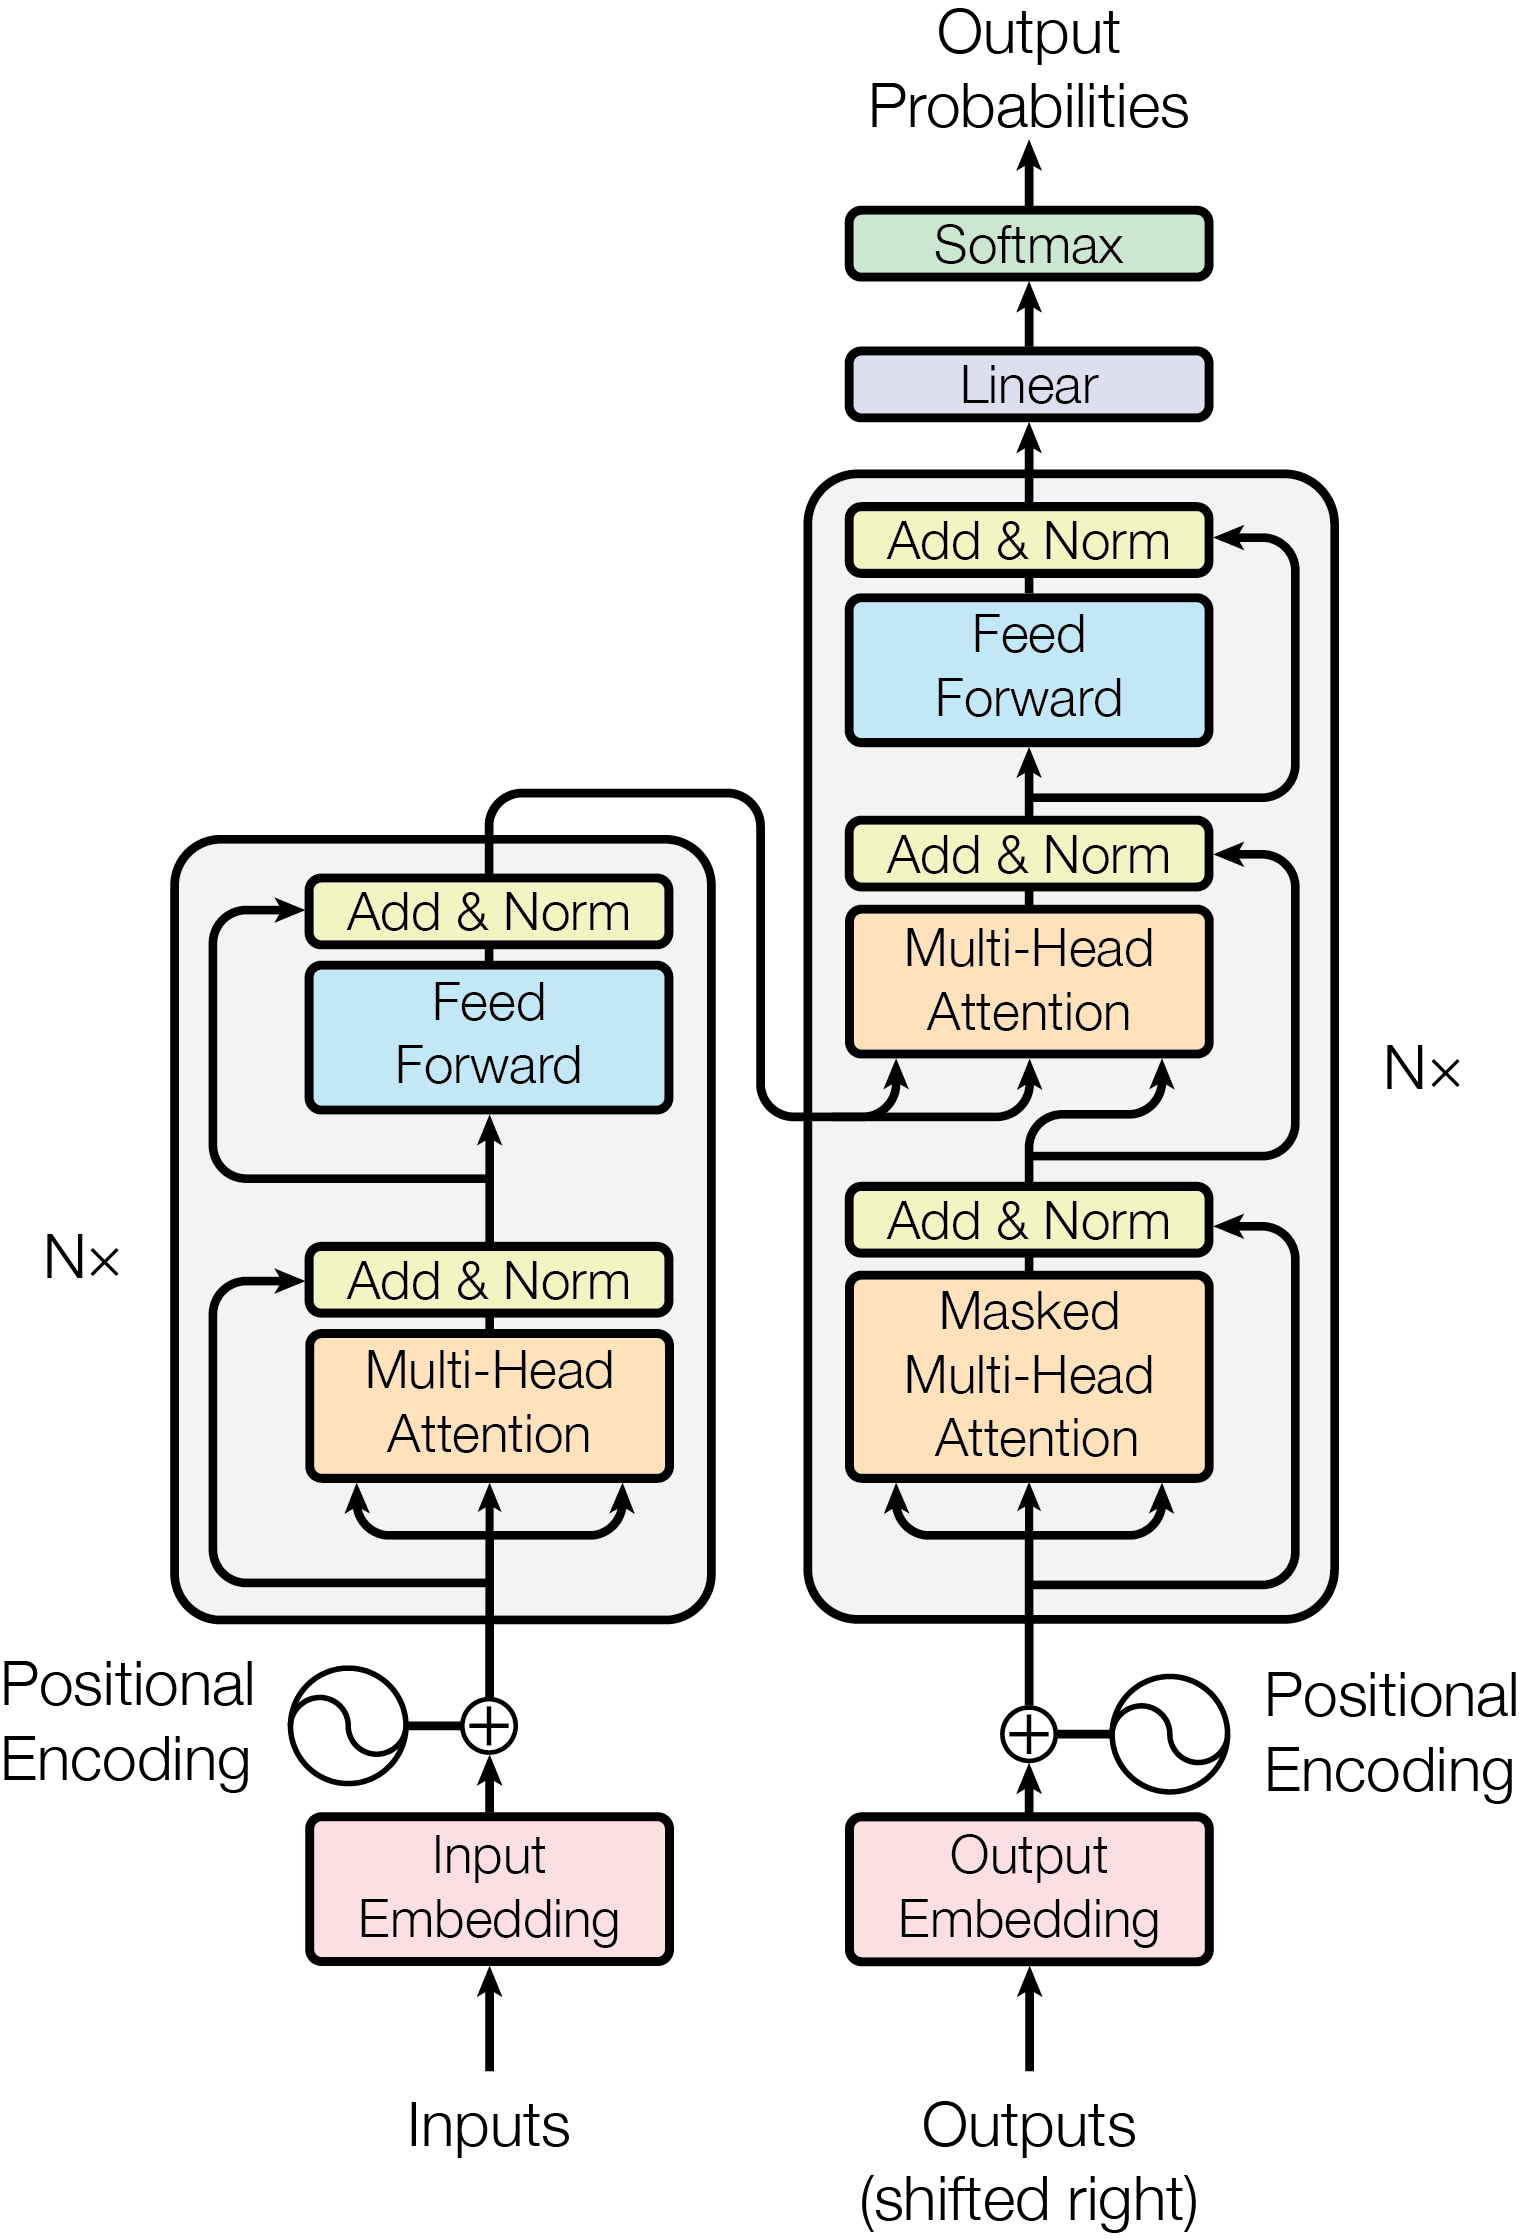
\includegraphics[scale=0.6]{./figures/ModalNet-21.png}
  \caption{The Transformer - model architecture.}
  \label{fig:model-arch}
\end{figure}


% LEAVE FOR FINAL REPORT
% \section{Results}
% Describe the performance of your model, either
% quantitatively or (for generative models) qualitatively. To
% help interpret the model, compare your model with a
% baseline model. Qualitative evaluation is OK.


% LEAVE FOR FINAL REPORT
% \section{Discussion}
% Interpret the results of your model. If appropriate,
% compare the model performance with the baseline.
% Discuss other features that you notice about the model.


% LEAVE FOR FINAL REPORT
% \section{Limitations}
% Describe some settings in which we’d expect your
% approach to perform poorly, or where all existing
% models fail. Try to guess or explain why these
% limitations are the way they are. Give some examples
% of possible extensions, ways to address these
% limitations or open problems

\section{Ethical considerations}
% Taha

% Potential ethical issues posed by the use or misuse of
% your model. Your report should transparently
% communicate the known or anticipated consequences
% of building and using machine learning models on this
% task.

% https://neurips.cc/public/EthicsGuidelines

\subsection{Ethical Issues}
One ethical consideration is the potential for the model to be used to cheat on math assignments/homework. This could encourage students to use the model as a shortcut rather than engaging with the material themselves, which would negatively impact a students capacity for critical thinking and problem-solving. 

Another ethical issue is intellectual property rights, as the model is trained on copyrighted data. The model could inadvertently promote plagiarism if it directly provides solutions that students submit as their own, without understanding the learning process. This could lead to academic dishonesty and undermine the integrity of the educational system.

\subsection{Mitigation Strategies}
To mitigate the first risk, the model should be used as a learning tool rather than a tool for cheating. For example, the model could be used to generate practice problems for students to solve, or to provide explanations for the solutions to problems. This would help students learn and improve their math skills, rather than using the model to cheat. Therefore, while automation can support learning, it is essential that it complements, rather than replaces, active engagement with the educational process.

To mitigate the second risk, the model should be used in a controlled environment where students are guided on how to use the model appropriately. For example, teachers could provide guidelines on how to use the model to check answers or generate practice problems, rather than using it to directly provide solutions. Furthermore, it is crucial to emphasize the value of understanding the material and using tools as aids rather than shortcuts. This would prevent plagiarism and encourage students to engage with the material and develop their problem-solving skills.

\section{Work division}

A description of how the work will be divided between
the team members, and how the team members will be
working together (e.g. meet every week Tuesday 4-5
pm).

Chloe - Background and Related Work, Abstract, Model Architecture

Takia - Model Architecture Figure, Model Architecture

Gabriel - Introduction, Model Architecture

Taha - Data, Ethical Considerations, Model Architecture

The team will work on each part, and meet every weekend for additional discussions. 

% LEAVE FOR FINAL REPORT
% \section{Conclusion}

% A description of how the work will be divided between
% the team members, and how the team members will be
% working together (e.g. meet every week Tuesday 4-5
% pm).

\bibliographystyle{unsrt}
\bibliography{references}

\end{document}